\chapter{Equazione del calore e metodo Perna-Malik}

\section{L'equazione del calore}

\raggedright

Prendiamo in esame l'equazione del calore

\begin{equation} 
\begin{cases}

\frac{\partial u}{\partial t}(t,x)-\Delta u(t,x) = 0 \ x \in \mathbb R^2, t\ge 0 \ .\\ 

u(0,x) = u_0(x)\ . \\

\end{cases}
\end{equation}

Prendiamo in esame l'eq del calore.

L'equazione del calore, come intuibile dal nome che porta, è stata formulata per determinare l'evoluzione di un sistema isolato che presenta al suo interno una data distribuzione di calore. E' banale pensare che con il passare del tempo il calore si distribuisca, tendendo per un tempo infinito ad una distribuzione uniforme.

\vspace{1em}

Euristicamente, non è difficile pensare che possiamo codificare (pensando ad un'immagine in bianco e nero) i pixel più luminosi come punti "più caldi" e quelli più scuri come punti "più freddi" ed applicare così l'equazione del calore.\\
Otteniamo quindi un'immagine sempre più "liscia", otteniamo di fatto una sfocatura, e per un numero di iterazioni idealmente infinito ci ritroveremmo con una distribuzione uniforme di colore, ossia una tinta unita.

\vspace{1em}

Vediamo con uno script matlab come opera nella pratica. \\
Per fare ciò operiamo una approssimazione alle differenze finite per il calcolo delle derivate. Questa si rifà molto alla definizione in se di derivata. Decidiamo quindi di approssimare \\
\vspace{2pt}
\centering 
$\frac{du}{dx} \approx \frac{u_i+1 - u_i}{delta(x)} $\\
\vspace{2pt}
\raggedright
Se la derivata seconda è la derivata della derivata, allora approssimiamo \\
\vspace{3cm}

\begin{table}[htp]              
\centering                      
\begin{tabular}%                
{r r}                  % parametri di incolonnamento: r (a destra), c (al centro), l (a sinistra),
								% p (per definire la larghezza della colonna)

$\frac{d^2u}{dx^2} \approx$ &
$\frac{
(\frac{u_i+1 - u_i}{\Delta(x)})_i+1 
- 
(\frac{u_i+1 - u_i}{\Delta(x)})_i
}{\Delta(x)}$

\\

\vline

\\
$=$ &
$\frac{
\frac{(u_i+1 - u_i)_i+1}{\Delta(x)} 
- 
\frac{(u_i+1 - u_i)_i}{\Delta(x)}
}{\Delta(x)}$

\\

\vline 

\\
$=$ &
$\frac{
\frac{(u_i+2 - u_i+1)}{\Delta(x)} 
- 
\frac{(u_i+1 - u_i)}{\Delta(x)}
}{\Delta(x)}$

\\

\vline 

\\
$=$ &
$\frac{
\frac{(u_i+2 - u_i+1) 
- 
(u_i+1 - u_i)}{\Delta(x)}
}{\Delta(x)}$

\\

\vline

\\
$=$ &
$\frac{
(u_i+2 - u_i+1) 
- 
(u_i+1 - u_i)}
{\Delta(x)^2}$

\\

\vline &
$\frac{
 u_i+2 - u_i+1 
-u_i+1 + u_i}
{\Delta(x)^2}$
\\

\end{tabular}
\end{table}



Per una migliore approssimazione è bene utilizzare un valore di delta(x) quanto più basso possibile. Il massimo che possiamo fare è vedere la differenza tra un pixel e quello adiacente ossia $\Delta(x)=1$, ma allora 
$$\frac{d^2u}{dx^2} \approx
\frac{
 u_i+2 - u_i+1 
-u_i+1 + u_i}
{\Delta(x)^2} = u_i+2 -2 u_i+1 + u_i$$
Capiamo che scorrendo tutti gli indici questo è equivalente a $u_i+1 -2 u_i + u_i-1.$

In sintesi utilizzeremo per il calcolo del laplaciamo l'approssimazione \\
\vspace{2pt}
\centering 
$\frac{d^2u}{dx^2} \approx u_i+1 -2 u_i + u_i-1$\\
\vspace{2pt}
\raggedright
Vediamo lo script:

\begin{lstlisting}


Im=imread('parrot.jpeg');   %Apro l'immmagine
Im=rgb2gray(Im);            %La trasformo in bianco e nero
Im = imnoise(Im,'gaussian');%Aggiungo del rumore

%---Definisco le costanti e le condizioni iniziali

[ny, nx, ~]=size(Im)        %Dimensioni dell'immagine
dt=0.25;                    %Passo temporale
u=double(Im);               %Copia dell'immagine originale su cui lavorare
T=3			    %Tempo, ossia T/dt + 1 definisce il numero di
                             iterazioni da eseguire
k=0.5;

%---Mostro l'immagine originale
imshow(uint8(Im))
title("immagine originale"); 

%---Metodo eq del calore
u=double(Im);
for t = 0:dt:T
   u_xx = u(:,[2:nx nx],:) - 2*u + u(:,[1 1:nx-1],:);  % derivata seconda lungo x
   u_yy = u([2:ny ny],:,:) - 2*u + u([1 1:ny-1],:,:);  % derivata seconda lungo y
   u= u + k*dt*(u_xx+u_yy);
   temp=u;
end

\end{lstlisting}
\vspace{1em}
Provando a cambiare il tempo, ossia il numero di iterazioni, osserviamo come un maggior lasso di tempo produca immagini più sfocate. 
Questo metodo però non è poi molto utile in generale, sì, il rumore viene eliminato o almeno ridotto ma si perdono importanti dettagli.\\

\begin{figure}[htb] 
\centering
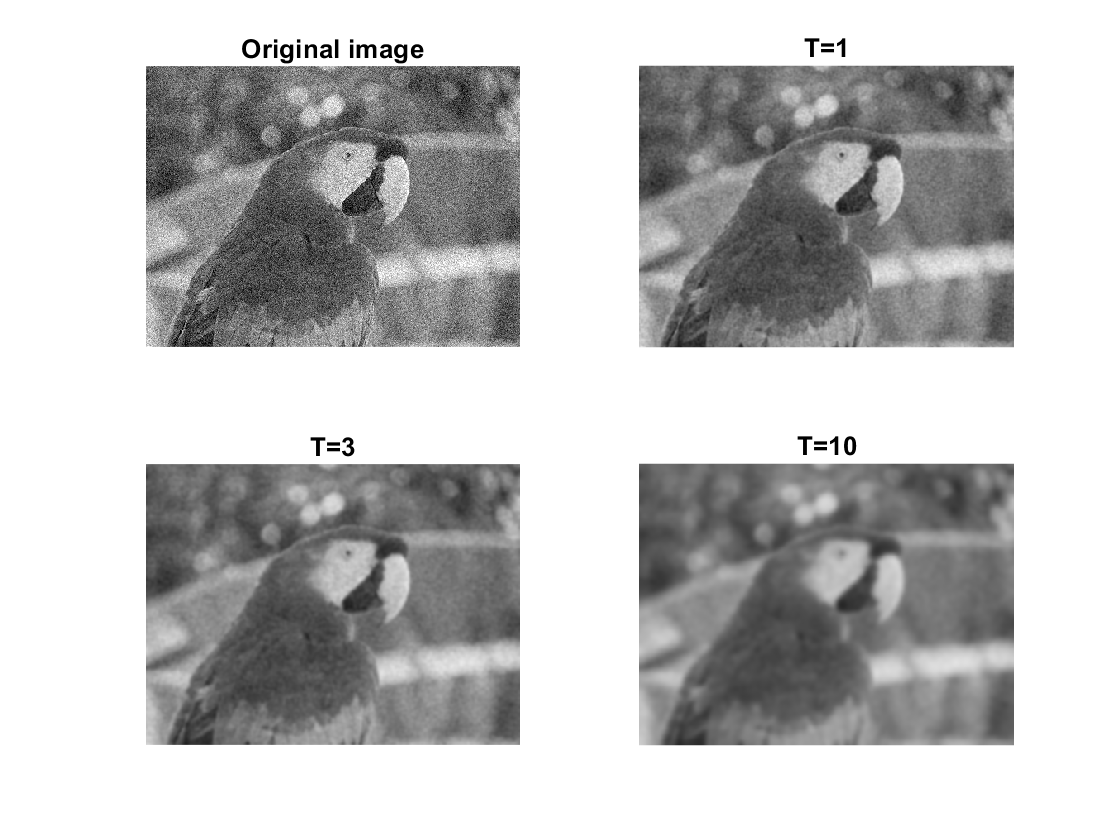
\includegraphics[scale=0.4]{Pictures/Risultati/eq del calore.png}
%\caption{Fiamme.}\label{fig:figura}
%\qquad\qquad
%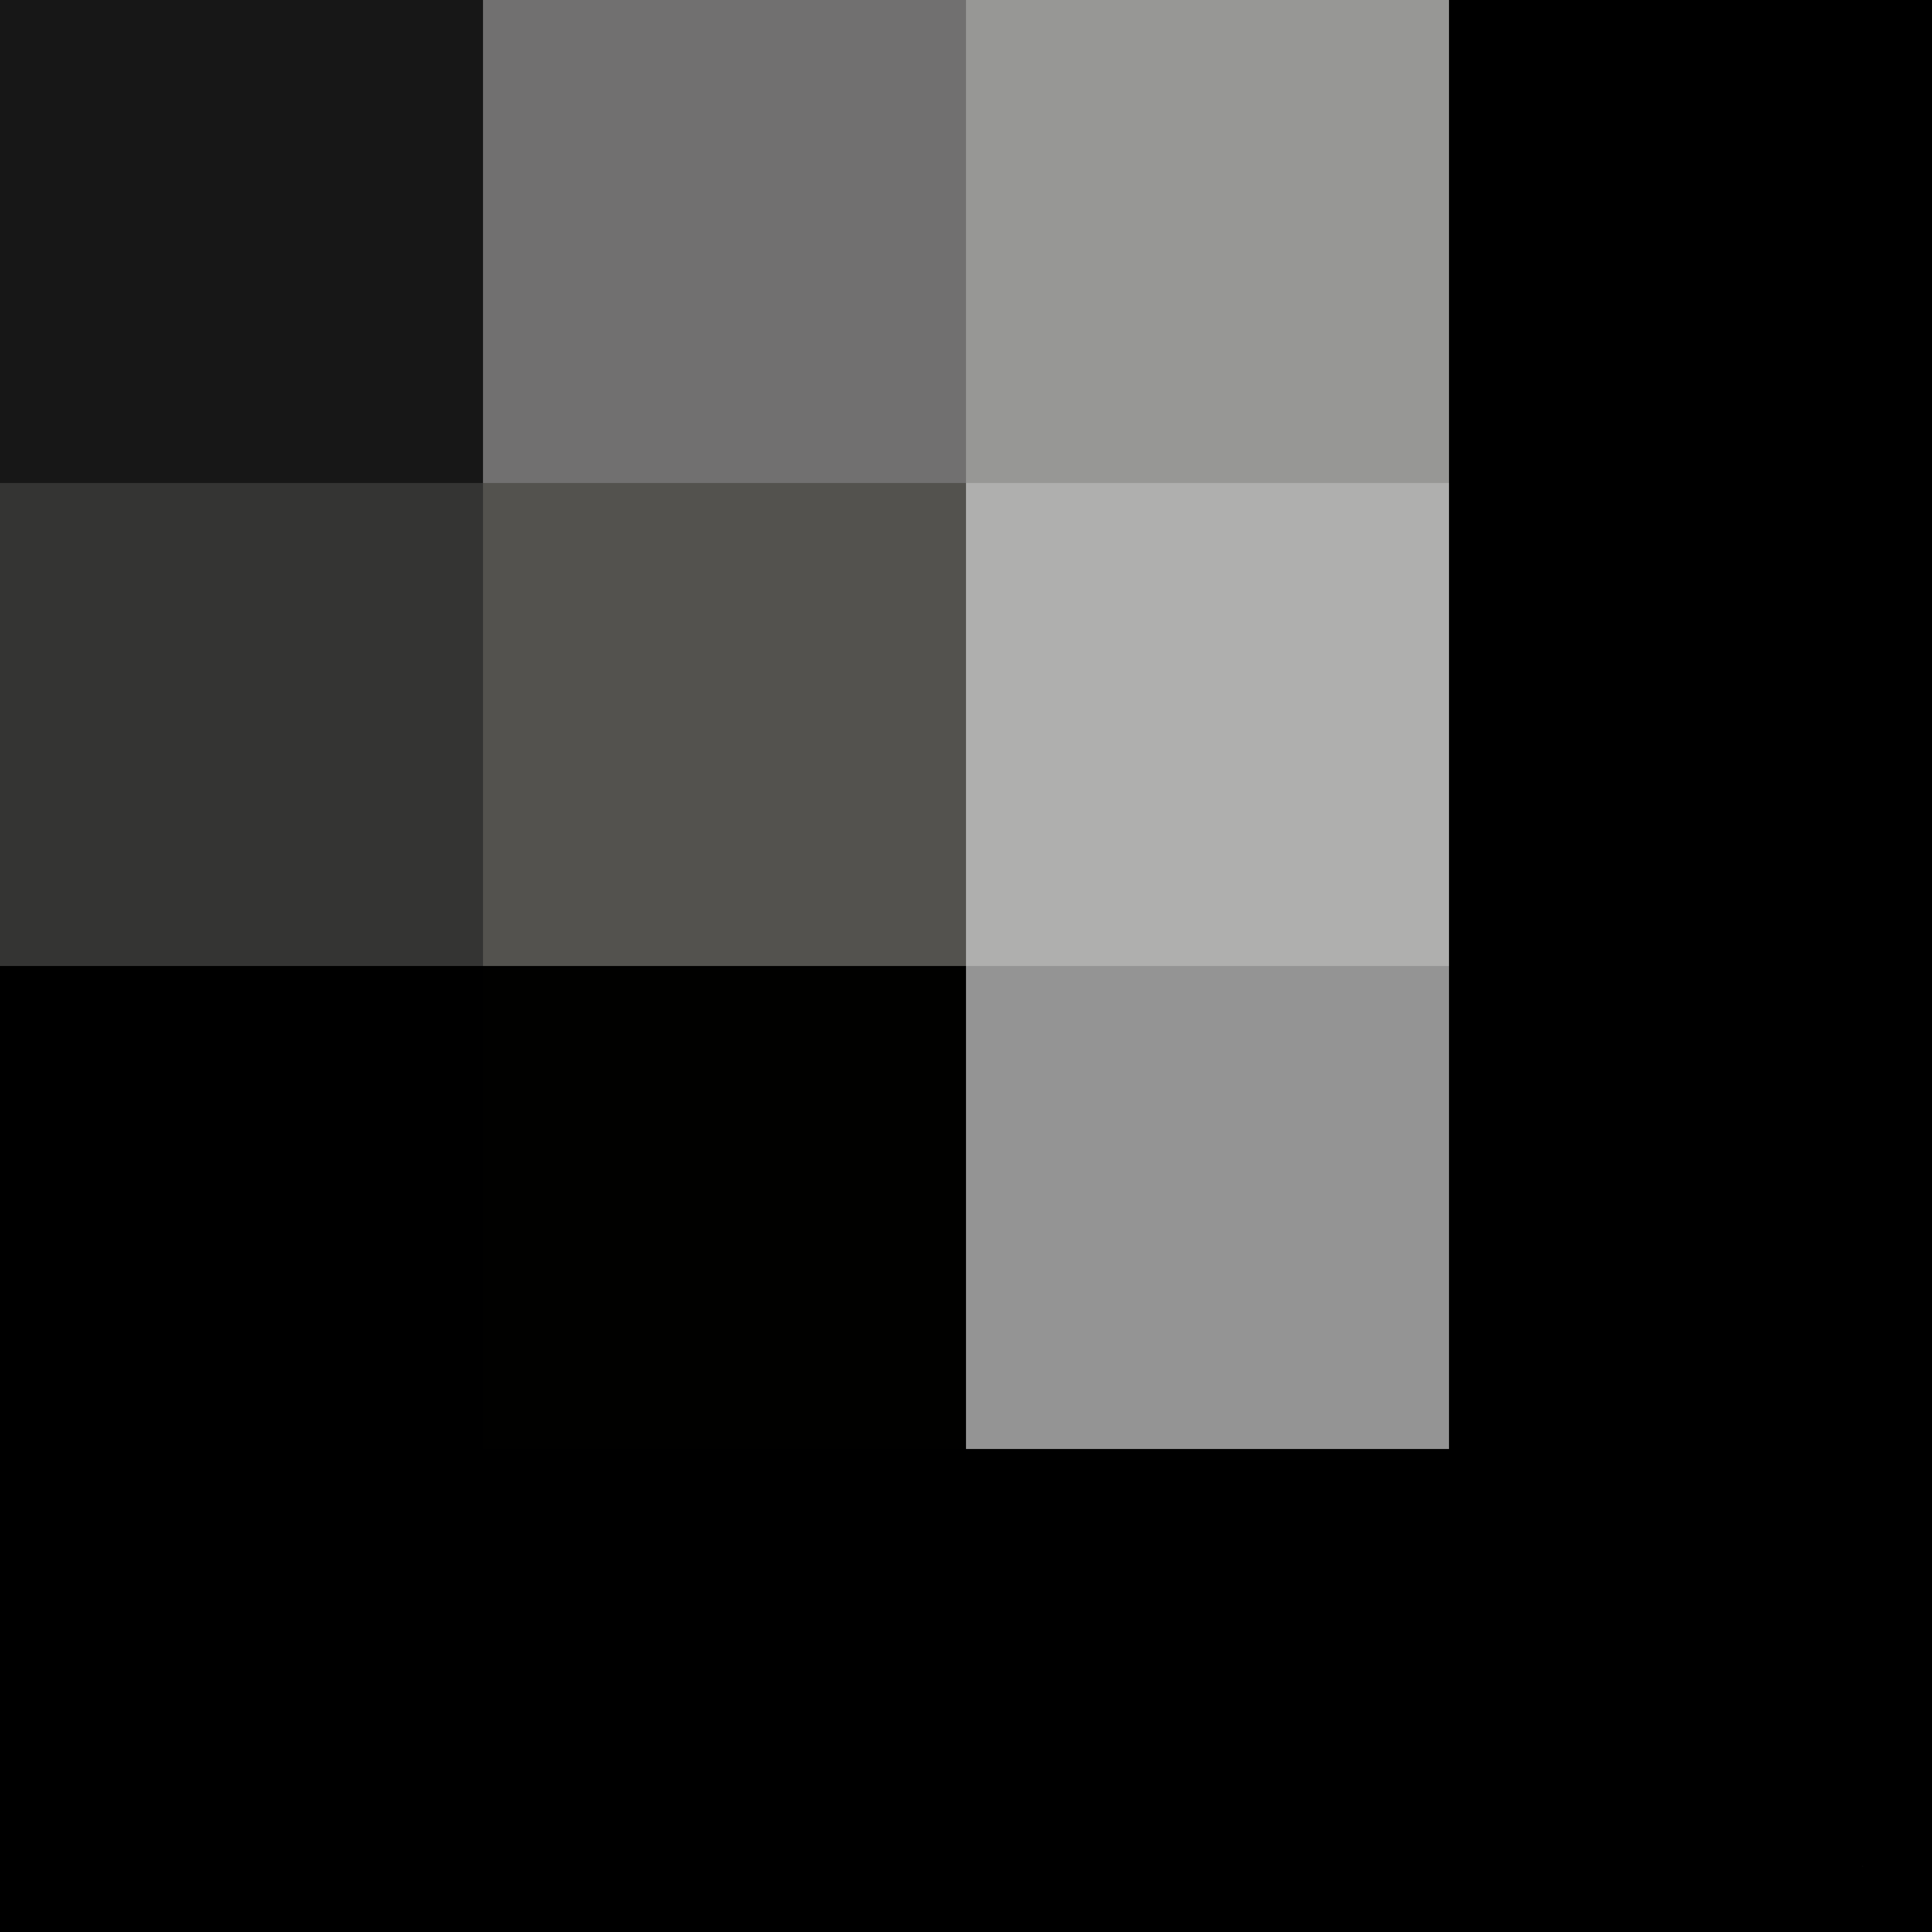
\includegraphics[scale=0.03]{Pictures/canvas8x8.png}
\caption{Effetti dell'eq del calore nel tempo.}\label{fig:figura}
\end{figure}

Operando una derivata in una data direzione, per il significato in sè di derivata, questa assume valori più elevati quando la variazione è elevata, e assume valori nulli quando non c'è variazione in quella direzione. Per questo motivo, applicata ad un' immagine, ne rileviamo i bordi!\\
Presa una tinta unita la derivata sarà quindi nulla in ogni suo punto (è intuitivo, se un'immagine è una funzione che, date due coordinate restituisce un colore, allora una tinta unita è una funzione costante ed in quanto tale ha derivata nulla).\\
\vspace{1em}
Operando una derivata seconda in una data direzione, per il significato in sè di derivata seconda, questa assume valori più elevati quando la concavità è più stretta, e assume valori pressocchè nulli quando non ci sono concavità (possiamo pensare alle concavità come a dei picchi o dei ventri, su di una immagine vuol dire chiazze di colore diverso).\\
Presa una sfumatura di colore che varia in maniera lineare, la derivata seconda sarà nulla in ogni suo punto, la derivata prima sarà invece costante. 
Scriviamo un piccolo script su MATLAB che ci mostri questo aspetto

\begin{lstlisting}
%---Operazioni preliminari
Im=imread("nome_immagine.png");	%Apro l'immmagine

[ny, nx, ~]=size(Im)        %Memorizzo le dimensioni dell'immagine
u=double(Im);               %Copia dell'immagine originale su cui lavorare
h=80;                       %Definisco un parametro che usero' per 
                             enfatizzare i bordi in fase di stampa 


%---Calcolo tutte le derivate
u_x =  u(:,[1 1:nx-1],:) - u;                       %derivata 
                                                     prima lungo x
u_xx = u(:,[2:nx nx],:) - 2*u + u(:,[1 1:nx-1],:);  %derivata 
                                                     seconda lungo x
u_y =  u([1 1:ny-1],:,:) - u;                       %derivata
                                                     prima lungo y
u_yy = u([2:ny ny],:,:) - 2*u + u([1 1:ny-1],:,:);  %derivata 
                                                     seconda lungo y
u_xy = u_x([1 1:ny-1],:,:) - u_x;                   %derivata 
                                                     seconda mista
   
%---Stampo i risultati
figure()
subplot(2,3,2),text(0.3,0,nome,"FontSize",20); axis off
subplot(2,3,4), imshow(Im)
title("Immagine originale")
subplot(2,3,5), imshow(uint8(h*abs(u_x)))
title("h*u_x")
subplot(2,3,6), imshow(uint8(h*abs(u_y)))
title("h*u_y")

figure()
subplot(2,3,2),text(0.3,0,nome,"FontSize",20); axis off
subplot(2,3,4), imshow(Im)
title("Immagine originale")
subplot(2,3,5), imshow(uint8(h*abs(u_x + u_y)))
title("h*(u_x + u_y)")
subplot(2,3,6), imshow(uint8(h*abs(u_xx + u_yy)))
title("h*(u_xx + u_yy)")
\end{lstlisting}

\vspace{6em}
Vediamo con diverse immagini molto semplici se otteniamo i risultati attesi.\\
%\vspace{1em}

\begin{figure}[htb] 
\centering
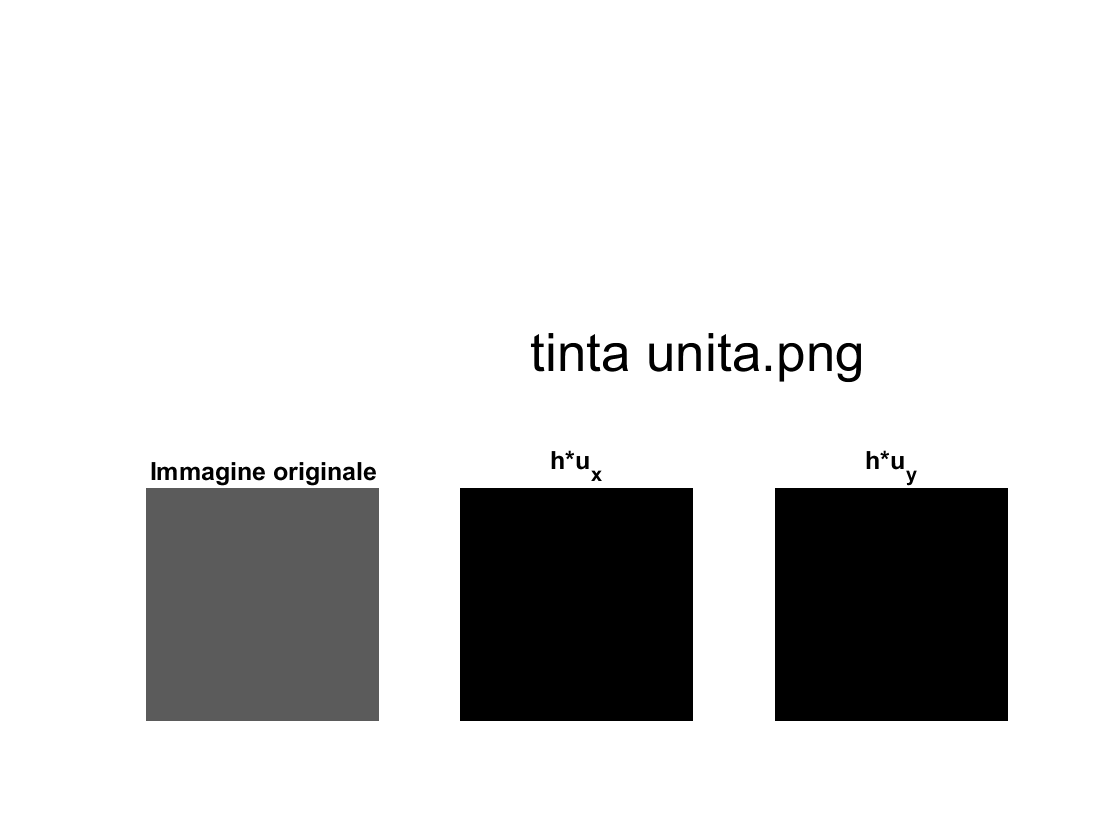
\includegraphics[scale=0.4, trim = 0 0 0 10.5cm, clip]{Pictures/Risultati/tinta unita bianco e nero derivate parziali.png}
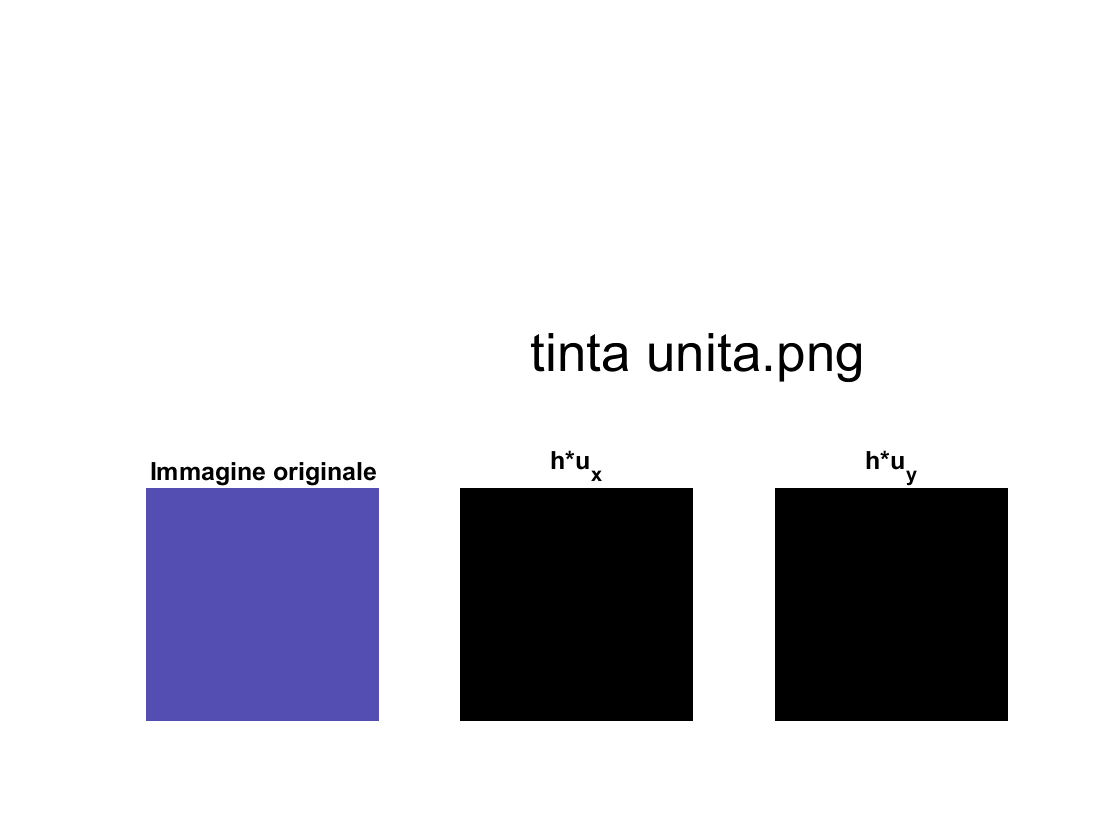
\includegraphics[scale=0.4, trim = 0 0 0 10.5cm, clip]{Pictures/Risultati/tinta unita derivate parziali.png}
\caption{Derivate parxiali di una tinta unita.}\label{fig:figura}
\end{figure}

Possiamo vedere come con un'immagine a tinta unita (che sia essa in bianco e nero o a colori) le derivate sono nulle, quindi lo saranno anche gradiente e laplaciano. Confermiamo inoltre che questi principi valgono sia a colori che in bianco e nero.\\

\newpage
\begin{figure}[htb] 
\centering
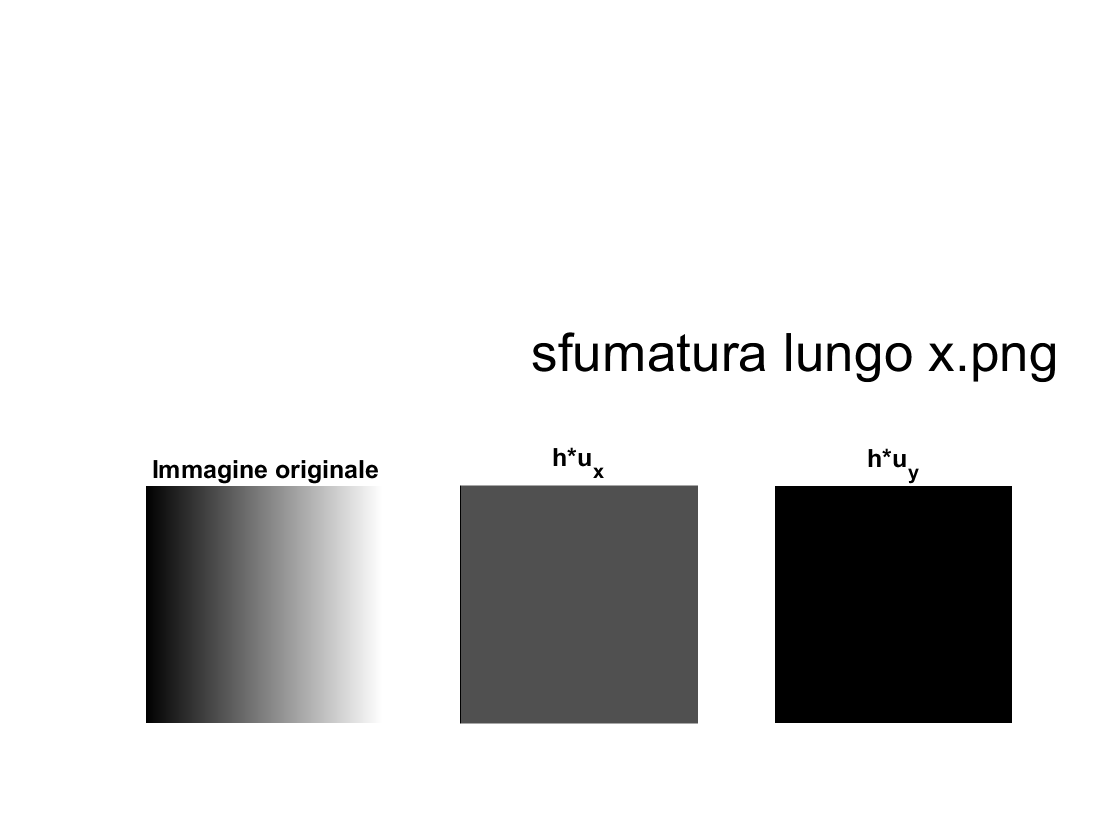
\includegraphics[scale=0.4, trim = 0 0 0 10.5cm, clip]{Pictures/Risultati/sfumatura lungo x bianco e nero derivate parziali.png}
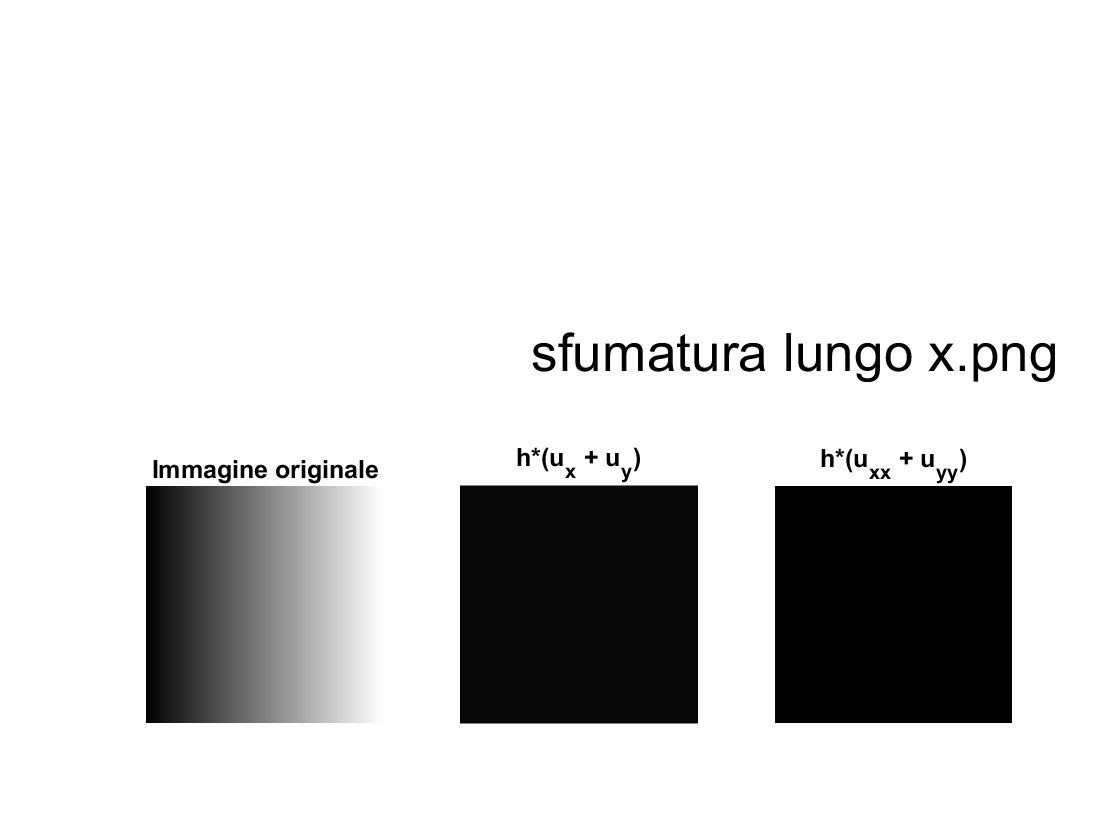
\includegraphics[scale=0.4, trim = 0 0 0 10.5cm, clip]{Pictures/Risultati/sfumatura lungo x bianco e nero gradiente e laplaciano.png}
\caption{Derivate parziali, gradiente e laplaciano di una sfumatura orizzontale.}\label{fig:figura}
\end{figure}

Guardando invece ad una immagine che presenta una sfumatura lineare lungo l'asse x, la derivata lungo x assume un valore costante mentre la derivata lungo y è nulla, proprio perchè lungo y non c'è variazione mentre lungo x c'è una variazione costante.\\
Ovviamente, date queste premesse, il gradiente sarà costante uguale $u_x$ (siccome $u_y=0$) e quindi il laplaciano sarà nullo.
Il fatto che in entrambi questi esempi il laplaciano sia nullo è un buon segno, lo useremo per rilevare i bordi ed in queste immagini non ve ne sono, quindi è giusto che il laplaciano sia nullo.\\

\newpage
\begin{figure}[htb] 
\centering
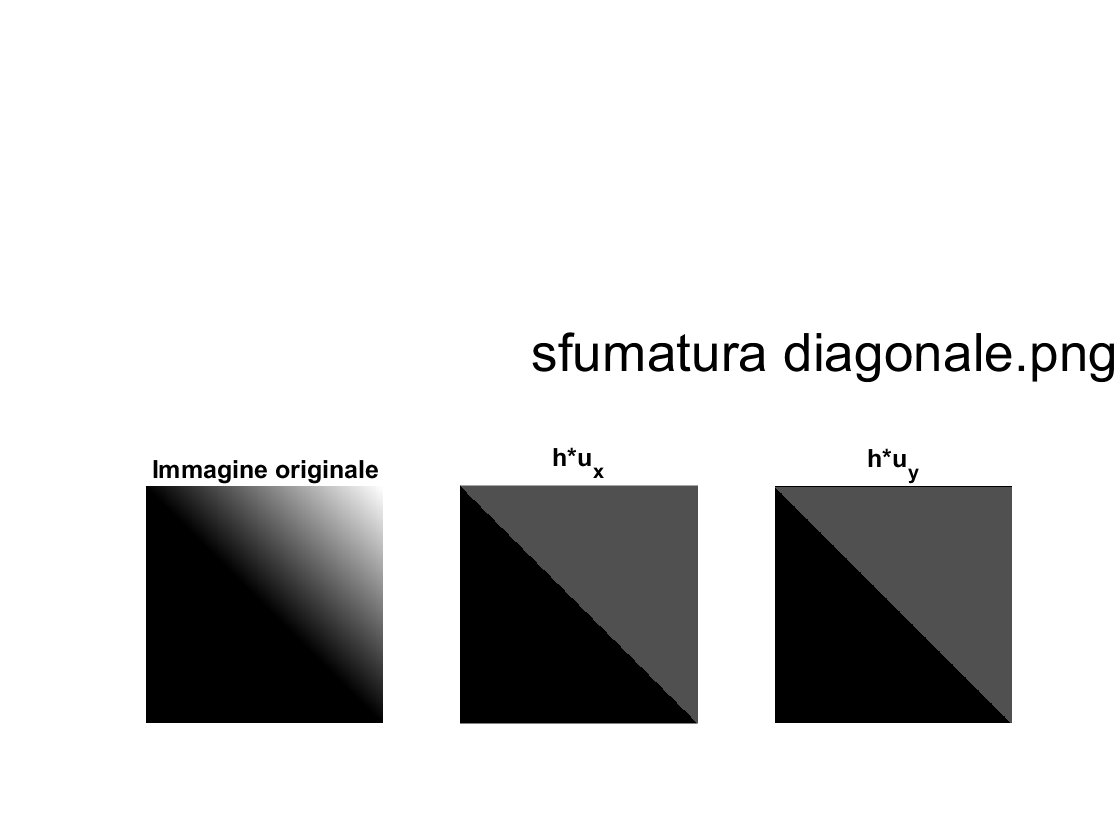
\includegraphics[scale=0.4, trim = 0 0 0 10.5cm, clip]{Pictures/Risultati/sfumatura diagonale bianco e nero derivate parziali.png}
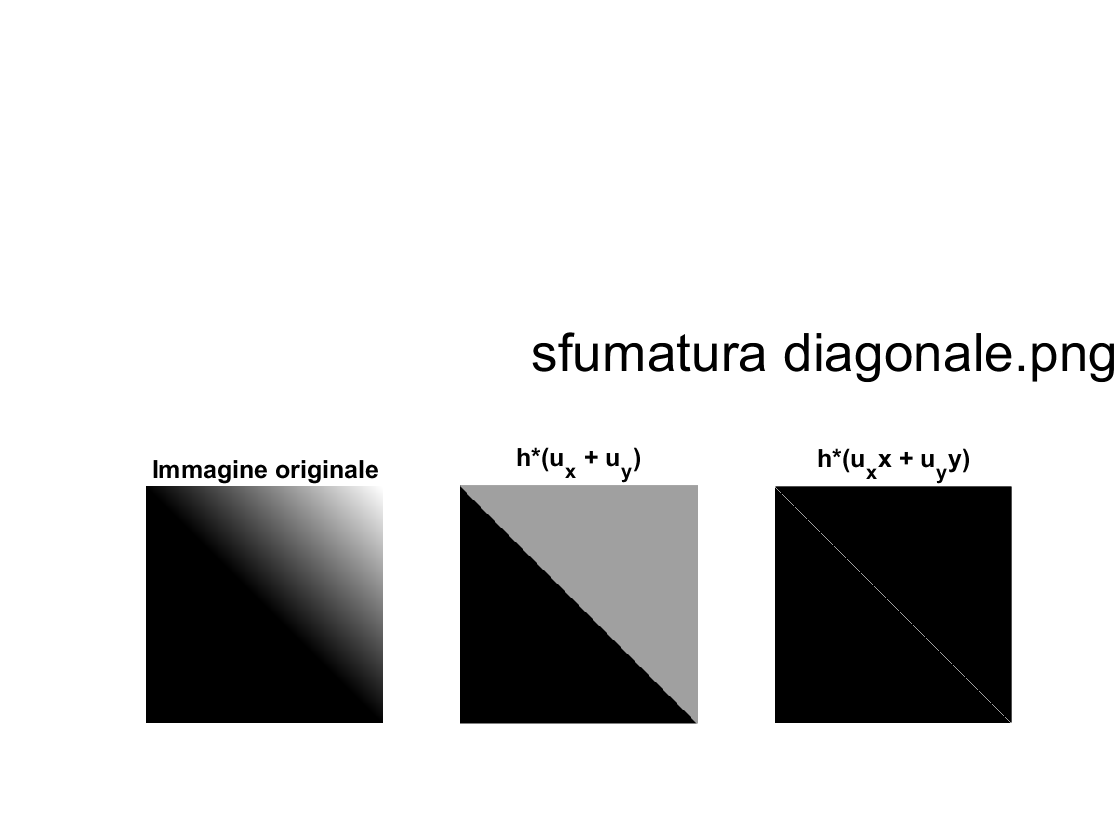
\includegraphics[scale=0.4, trim = 0 0 0 10.5cm, clip]{Pictures/Risultati/sfumatura diagonale bianco e nero gradiente e laplaciano.png}
\caption{Derivate parziali, gradiente e laplaciano di una sfumatura diagonale.}\label{fig:figura}
\end{figure}

Se prendiamo una sfumatura diagonale ma solo su metà immagine vediamo dei riultati interessanti: entrambe le derivate parziali sono nulle nelle regioni in cui non c'è sfumatura, esattamente come nel caso della tinta unita, ed entrambe sono costanti dove c'è sfumatura (che ricordiamo essere lineare).\\
Tutto ciò riconferma quanto visto dai punti precedenti, decidiamo quindi di volgere uno sguardo al gradiente ed al laplaciano e noteremo qualcosa di interessante, il gradiente ha un aspetto molto simile alle due derivate parziali, sommando i loro valori è semplicemente più luminoso.\\
Per quanto riguarda il gradiente la storia cambia. Le derivate seconde sono indicatrici della variazione delle derivate prime, cioè della variazione della variazione del valore della funzione, ma l'unica variazione che hanno le derivate prime è lungo la diagonale.
Abbiamo così individuato il nostro primo bordo, cioè la diagonale che divide di fatto due regioni, una in cui il colore è costante ed una in cui sfuma.\\

\vspace{1em}

Facciamo ancora un esempio, proviamo ad introdurre una semplice figura e vediamo cosa accade.\\

\newpage
\begin{figure}[htb] 
\centering
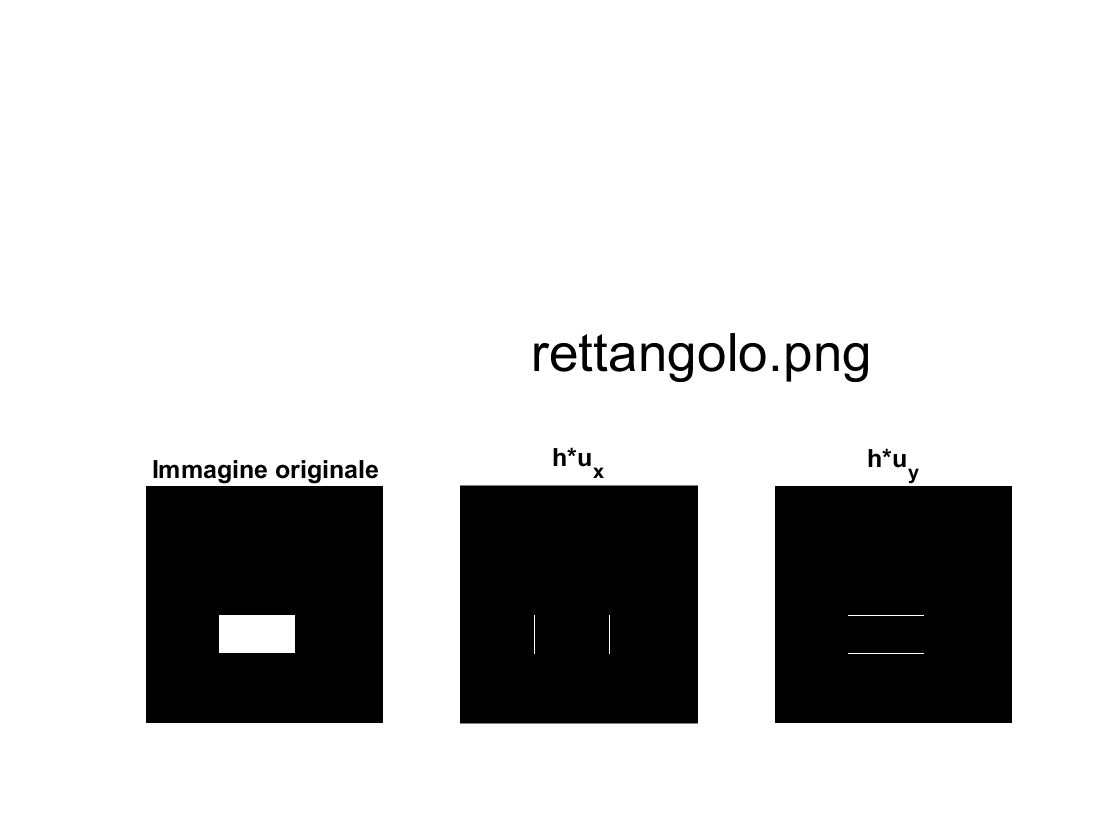
\includegraphics[scale=0.4, trim = 0 0 0 10.5cm, clip]{Pictures/Risultati/rettangolo bianco e nero derivate parziali.png}
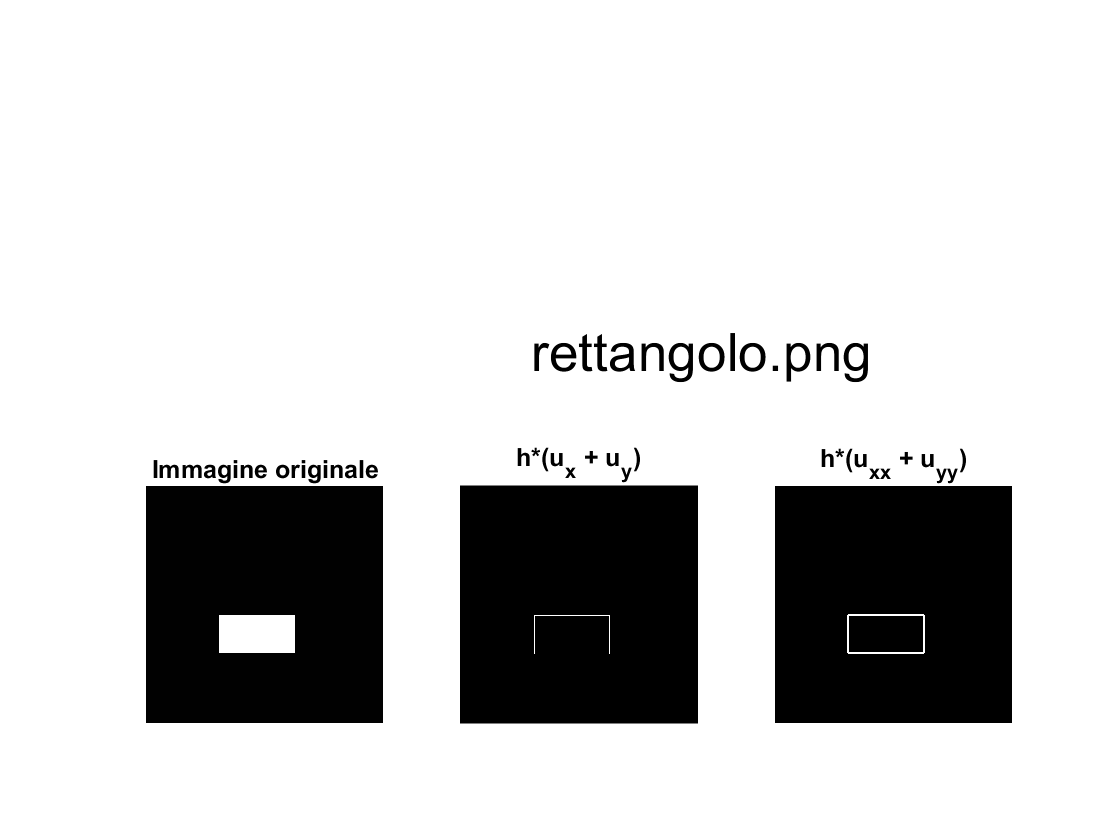
\includegraphics[scale=0.4, trim = 0 0 0 10.5cm, clip]{Pictures/Risultati/rettangolo bianco e nero gradiente e laplaciano.png}
\caption{Derivate parziali, gradiente e laplaciano di una figura semplice.}\label{fig:figura}
\end{figure}

Abbiamo importato un rettangolo nero su di uno sfondo bianco, come confermato anche dalla prima sfumatura, la derivata lungo x rileva i bordi verticali, quella lungo y i bordi orizzontali, dalla loro somma (quindi dal gradiente) otteniamo già il bordo del rettangolo.
Il bordo così ottenuto è un bordo che idealmente rimarrà inalterato a prescindere dall'ordine della derivata, in particolare quindi anche per derivate seconde, quindi il laplaciano continua a soddisfare la nostra richiesta di determinare i bordi. \\
Come detto: "Il bordo così ottenuto è un bordo che idealmente rimarrà inalterato a prescindere dall'ordine della derivata" cerchiamo di capire perchè. Presa una striscia di pixel, cioè uno strato della nostra immagine (immaginiamola quindi come una funzione da R in R), otterremo quindi una funzione porta!\\
La funzione porta non è derivabile in senso classico, ripensando alla definizione di derivata avremmo un valore di +infinito prima e -infinito poi. La sua derivata sarà quindi una coppia di delta di Dirac\\

